%%
%% This is file `mitsample.tex',
%% generated with the docstrip utility.
%
% The original source files were:
%
% ubcthesis.dtx  (with options: `mitsampletex')
%% 
%% This file was generated from the ubcthesis package.
%% --------------------------------------------------------------
%% 
%% Copyright (C) 2001
%% Michael McNeil Forbes
%% mforbes@alum.mit.edu
%% 
%% This file may be distributed and/or modified under the
%% conditions of the LaTeX Project Public License, either version 1.2
%% of this license or (at your option) any later version.
%% The latest version of this license is in
%%    http://www.latex-project.org/lppl.txt
%% and version 1.2 or later is part of all distributions of LaTeX
%% version 1999/12/01 or later.
%% 
%% This program is distributed in the hope that it will be useful,
%% but WITHOUT ANY WARRANTY; without even the implied warranty of
%% MERCHANTABILITY or FITNESS FOR A PARTICULAR PURPOSE.  See the
%% LaTeX Project Public License for more details.
%% 
%% This program consists of the files ubcthesis.dtx, ubcthesis.ins, and
%% the sample figures fig.eps and fig.fig.
%% 
%% This file may be modified and used as a base for your thesis without
%% including the licence agreement as long as the content (i.e. textual
%% body) of the file is completely rewritten. You must, however, change
%% the name of the file.
%% 
%% This file may only be distributed together with a copy of this
%% program. You may, however, distribute this program without generated
%% files such as this one.
%% 

% This Sample thesis requires \LaTeX2e
\NeedsTeXFormat{LaTeX2e}[1995/12/01]
\ProvidesFile{mitsample.tex}[2012/04/07 v1.70 ^^J
 Massachusetts Institute of Technology Sample Thesis]

\documentclass[msc,10pt,oneside]{mitthesis}
%
% To compile issue the following commands:
% latex mitsample
% bibtex mitsample
% latex mitsample
% latex mitsample
% latex mitsample
%
% To view use xdvi (on unix systems):
% xdvi mitsample.dvi
%
% To make a postscript file, use dvips:
% dvips -o mitsample.ps mitsample.dvi
%
% To view the postscript file, use ghostview or gv (on unix systems):
% gv mitsample.ps
%
%************************************************
% Optional packages.
%
% The use of these packages is optional: they are standard now and
% should be installed on your system, but if they are not, you might
% have to comment out the appropriate lines to get this file to
% compile.
%
%******** natbib ********************************
% This is a very nice package for bibliographies.  It includes options
% for sorting and compressing bibliographic entries.
\usepackage[numbers,sort&compress]{natbib}

%******** graphics and graphicx ******************************
% This allows you to include encapsulated postscript files.  If you
% don't have this, comment the \includegraphics{} line following the
% comment "%includegraphics" later in this file.
\usepackage{graphicx}

%******** pdflscape ********************************
% This allows you to include landscape layout pages by using the
% |landscape| environment.  The use of |pdflscape| is preferred over
% the standard |lscape| package because it automatically rotates the
% page in the pdf file for easier reading.  (Thanks to Joseph Shea
% for pointing this out.)
\usepackage{pdflscape}

%******** psfrag ******************************
% This allows you to replace text in postscript pictures with formated
% latex text.  This allows you to use math in graph labels
% etc. Uncomment the psfrag lines following the "%psfrag" comment
% later in this file if you don't have this package.  The replacements
% will only be visible in the final postscript file: they will be
% listed in the .dvi file but not performed.
\usepackage{psfrag}

%******** afterpage ***************************
% This package allows you to issue commands at the end of the current
% page.  A good use for this is to use the command
% \afterpage{\clearpage} right after a figure.  This will cause the
% figure to be inserted on the page following the current one (or on
% the current page if it will fit) but will not break the page in the
% middle.
\usepackage{afterpage}

%******** hyperref *****************************
% Please read the manual:
% http://www.tug.org/applications/hyperref/manual.html
%
% This adds hyperlinks to your document: with the right viewers (later
% versions of xdvi, acrobat with pdftex, latex2html etc.) this will
% make your equation, figure, citation references etc. hyperlinks so
% that you can click on them.  Also, your table of contents will be
% able to take you to the appropriate sections.  In the viewers that
% support this, the links often appear with an underscore.  This
% underscore will not appear in printed versions.
%
% Note: if you do not use the hypertex option, then the dvips driver
% may be loaded by default.  This will cause the entries in the list
% of figures and list of tables to be on a single line because dvips
% does not deal with hyperlinks on broken lines properly.
%
% NOTE: HYPERREF is sensitive to the ORDER in which it is LOADED.
% For example, it must be loaded AFTER natbib but BEFORE newly
% defined float environments.  See the README file with the hyperref
% for some help with this.  If you have some very obscure errors, try
% first disabling hyperref.  If that fixes the problem, try various
% orderings.
%
% Note also that there is a bug with versions before 2003/11/30
% v6.74m that cause the float package to not function correctly.
% Please ensure you have a current version of this package.  A
% warning will be issued if you leave the date below but do not have
% a current version installed.
%
% Some notes on options: depending on how you build your files, you
% may need to choose the appropriate option (such as [pdftex]) for the
% backend driver (see the hyperref manual for a complete list).  Also,
% the default here is to make links from the page numbers in the table
% of contents and lists of figures etc.  There are other options:
% excluding the [linktocpage] option will make the entire text a
% hyperref, but for some backends will prevent the text from wrapping
% which can look terrible.  There is a [breaklinks=true] option that
% will be set if the backend supports (dvipdfm for example supports
% it but does not work with psfrag.)
%
% Finally, there are many options for choosing the colours of the
% links.  These will be included by default in future versions but
% you should probably consider changing some now for the electronic
% version of your thesis.
\usepackage[unicode=true,
  linktocpage,
  linkbordercolor={0.5 0.5 1},
  citebordercolor={0.5 1 0.5},
  linkcolor=blue]{hyperref}

% If you would like to compile this sample thesis without the
% hyperref package, then you will need to comment out the previous
% \usepackage command and uncomment the following command which will
% put the URL's in a typewriter font but not link them.
%\newcommand\url[1]{\texttt{#1}}

% These commands are optional.  The defaults are shown.
\institution{Massachusetts Institute of Technology}
\institutionaddress{Cambridge}
\program{Physics}

% You can issue as many of these as you have...
\previousdegree{B.Sc., The University of British Columbia, 1999}
\previousdegree{M.Sc., The University of British Columbia, 2001}

% You can override the option setting here.
% \degreetitle{Jack of All Trades}

% These commands are required.
\title{A Sample Thesis}
\subtitle{With a Subtitle}
\author{Michael M$^{\rm c}$Neil Forbes}
\copyrightyear{2000}
\submitdate{June 2004}

% These commands are required by MIT.
\advisor{Frank Wilczek}
\advisortitle{Herman Feshbach Professor of Physics}
\chairman{Thomas Greytak}{Professor and Associate Department Head for
  Education}
% One might want to override the format of the section and chapter
% numbers.  This shows you how to do it.  Note that
\renewcommand\thepart         {\Roman{part}}
\renewcommand\thechapter      {\arabic{chapter}}
\renewcommand\thesection      {\thechapter.\arabic{section}}
\renewcommand\thesubsection   {\thesection.\arabic{subsection}}
\renewcommand\thesubsubsection{\thesubsection.\arabic{subsubsection}}
\renewcommand\theparagraph    {\thesubsubsection.\arabic{paragraph}}
\renewcommand\thesubparagraph {\theparagraph.\arabic{subparagraph}}

\setcounter{tocdepth}{2}
\setcounter{secnumdepth}{2}

% Here is the start of the document.
\begin{document}

% Unlike the UBC thesis, page numbering for MIT theses should start
% at 1 and continue.  Thus, there is no \frontmatter command issued
% here as there was for the UBC thesis.

\maketitle
\authorizationform
\begin{abstract}
  The \texttt{genthesis.cls} \LaTeX{} class file and accompanying
  documents, such as this sample thesis, are distributed in the hope
  that it will be useful but without any warranty (without even the
  implied warranty of fitness for a particular purpose).  For a
  description of this file's purpose, and instructions on its use, see
  below.

  These files are distributed under the GPL which should be included
  here in the future.  Please let the author know of any changes or
  improvements that should be made.

  Michael Forbes.
  mforbes@alum.mit.edu
\end{abstract}

\tableofcontents
\listoftables
\listoffigures
% Any other lists should come here, i.e.
% Abbreviation schemes, definitions, lists of formulae, list of
% schemes, etc.

\chapter{Preface}
These papers have been published earlier\ldots.

\chapter{Acknowledgements}
Thank you mother here.

% Force a new page.
\newpage

% Any other unusual sections should come here between the
% acknowledgements and the main body.

% Suppress the running headers for this page only.
\thispagestyle{plain}
\chapter*{Disclaimer} % Unnumbered
The \texttt{mitthesis} \LaTeX{} class and the accompanying sample files
are \emph{unofficial} and are not supported by the Massachusetts
Institute of Technology.  While I have attempted to make the style
file and sample files conform to all of the requirements set forth by
the library, you should always consult one of the library staff
members for assistance with problems \emph{before} starting final
draft.  You should be able to find the thesis requirements at one of
the following sites:
\begin{table}[h]
  \begin{center}
    \begin{tabular}{|l|}
      \hline
      \url{http://libraries.mit.edu/archives/thesis-specs/}\\
      \url{http://libraries.mit.edu/archives/index.html}\\
      \hline
    \end{tabular}
  \end{center}
  \caption{\label{tab:ubcurls}
    Potential sources of information regarding thesis preparation at MIT.}
\end{table}

% Force a new page.
\newpage

% Suppress the running headers for this page only.
\thispagestyle{plain}

% Here we provide a short optional argument to \chapter[]{}.  This
% optional argument will appear in the table of contents.  For long
% titles, one should use this to give a single-line entry to the
% table of contents.
\chapter[Poem]{A Japanese Introduction}

% Here is a quote:
\begin{quote}
  % It is centered
  \begin{center}
    This is a small poem,\\
    a little poem, a Haiku,\\
    to show you how to.\\
    ---Michael Forbes.
  \end{center}
\end{quote}
This small poem shows several features:
\begin{itemize}
\item The \verb|\newpage| command has been used to force a page break.
\item The pagestyle has been set to suppress the headers using the
  command \verb|\thispagestyle{plain}|.  Note that using
  \verb|\pagestyle{plain}| would have affected all of the subsequent
  pages.
\item The \verb|\chapter[Poem]{A Japanese Introduction}| command has
  been used with an optional argument to generate a title and to list
  this ``chapter'' in the table of contents as ``Poem''.  If one did
  not desire to have an entry in the table of contents, then one would
  just use the starred command \verb|\chapter*{}|.  The use of an
  optional argument is useful for long chapter and section titles that
  take up too much space in the table of contents.
\end{itemize}

% Parts are the largest units
\part{Thesis}

% Chapters are the next main unit.
\chapter{This is a Chapter}

% Sections are a sub-unit
\section{A Section}
Here is a section with some text.  Equations look like this $y=x$.

This is an example of a second paragraph in a section so you can
see how much it is indented by.

% Subsections follow
\subsection{This is a Subsection}
Here is an example of a citation: \cite{Forbes:2006ba}.  The actual
form of the citation is governed by the bibliographystyle.  These
citations are maintained in a BIBTeX file \texttt{sample.bib}.  You
could type these directly into the file.  For an example of the format
to use look at the file \texttt{mitsample.bbl} after you compile this
file.

This is an example of a second paragraph in a subsection so you can
see how much it is indented by.

\subsubsection{This is a Subsubsection}
Here are some more citations \cite{LL3:1977,Peccei:1989,Turner:1999}.
If you use the \texttt{natbib} package with the \verb+sort&compress+
option, then the following citation will look the same as the first
citation in this section: \cite{Turner:1999,Peccei:1989,LL3:1977}.

This is an example of a second paragraph in a subsubsection so you can
see how much it is indented by.

\paragraph{This is a Paragraph}
Paragraphs and subparagraphs are the smallest units of text.  There is
no subsubsubsection etc.

\subparagraph{This is a Subparagraph}
This is the last level of organisation.  If you need more than this,
you should consider reorganizing your work\dots

\begin{equation}
  \mathrm{f}(x)=\int_{-\infty}^{\int_{-\infty}^x
    e^{-\frac{y^2}{2}}\mathrm{d}{y}}e^{-z^2}\mathrm{d}z
\end{equation}

In order to show you what a separate page would look like (i.e. without
a chapter heading) I must type some more text.  Thus I will babble a
bit and keep babbling for at least one more page\ldots  What you
should notice is that the chapter titles appear substantially lower
than the continuing text. Babble babble
babble babble babble babble babble babble babble babble babble babble
babble babble babble babble babble babble babble babble babble babble
babble babble babble babble babble babble babble babble babble babble
babble babble babble babble babble babble babble babble babble.

Babble babble babble babble babble babble babble babble babble babble
babble babble babble babble babble babble babble babble babble babble
babble babble babble babble babble babble babble babble babble babble
babble babble babble babble babble babble babble babble babble babble
babble babble babble babble babble babble babble babble babble babble
babble babble babble babble babble babble babble babble babble babble
babble babble babble babble babble babble babble babble babble babble
babble babble babble babble babble babble babble babble babble babble
babble babble babble babble babble babble babble babble babble babble
babble babble babble babble babble babble babble babble babble babble
babble babble babble babble babble babble babble babble babble babble
babble babble babble babble babble babble babble babble babble babble
babble babble babble babble.

\begin{table}[t]                 %optional [t, b or h];
  \begin{tabular}{|r||r@{.}l|}
    \hline
    Phoenix & \$960&35\\
    \hline
    Calgary & \$250&00\\
    \hline
  \end{tabular}
  \caption{
    \label{tab:Table1}
    Here is the caption for this wonderful table.Text of Caption}
\end{table}

\chapter[Another Chapter\ldots]{Another Chapter with a Very Long
  Chapter-name that will Probably Cause Problems}
This chapter name is very long and does not display properly in the
running headers or in the table of contents.  To deal with this, we
provide a shorter version of the title as the optional argument to the
\verb|\chapter[]{}| command.

\section{Another Section}
Another bunch of text to demonstrate what this file does.
You might want a list for example:
\begin{itemize}
\item An item in a list.
\item Another item in a list.
\end{itemize}

\section*{An Unnumbered Section That is Not Included in the Table of
  Contents}
%% We would like to place the figure here, so we start with [h].
%% Note that we have located the figure between paragraphs (rather,
%% before one) so that it does not split up sentences.
\begin{figure}[ht]
  \begin{center}
%% psfrag: comment the following line if not using the psfrag package
    \psfrag{pie makes me happy!}{$\pi$ makes me happy!}
%% includegraphics: comment the following if not using the graphicx package
    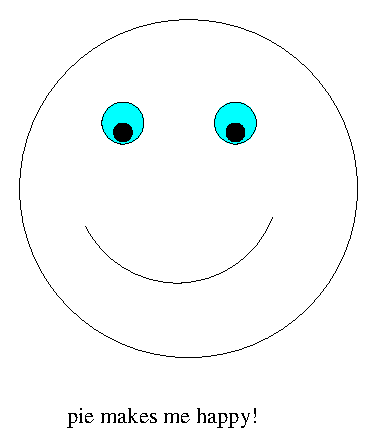
\includegraphics[width=0.4\textwidth]{fig.eps}
    \caption[Happy Face: figure example.]{\label{fig:happy} This is a
      figure of a happy face with a \texttt{psfrag} replacement.  The
      original figure (drawn in xfig and exported to a .eps file) has
      the text ``pie makes me happy!''.  The \texttt{psfrag} package
      replaces this with ``$\pi$ makes me happy!''.  Note that we have
      used the optional argument for the caption command so that only
      a short version of this caption occurs in the list of figures.}
  \end{center}
\end{figure}
\afterpage{\clearpage}
Here is an example of a figure environment.
Perhaps I should say that the example of a figure can be seen in
Figure~\ref{fig:happy}.  Figure placement can be tricky with \LaTeX\
because figures and tables are treated as ``floats'': text can flow
around them, but if there is not enough space, they will appear later.
To prevent figures from going too far, the
\verb|\afterpage{\clearpage}| command can be used.  This makes sure
that the figure are typeset at the end of the page (possibly appear on
their own on the following pages) and before any subsequent text.

The \verb|\clearpage| forces a page break so that the figure can be
placed, but without the the \verb|\afterpage{}| command, the page
would be broken too early (at the \verb|\clearpage| statement).  The
\verb|\afterpage{}| command tells \LaTeX{} to issue the command after
the present page has been rendered.

Be careful when using the ``here'' placement option
\verb|\begin{figure}[ht]| that you place the figure between paragraphs
in your text, otherwise \LaTeX{} might actually insert it in the
middle of a sentence (which does not look very good and is frowned
upon by the editors!)

\subsection*{An Unnumbered Subsection}
Note that if you use subsections or further divisions under an
unnumbered section, then you should make them unnumbered as well
otherwise you will end up with zeros in the section numbering.

\chapter{Landscape Mode}
The landscape mode allows you to rotate a page through 90 degrees.  It
is generally not a good idea to make the chapter heading landscape,
but it can be useful for long tables etc.

\begin{landscape}
  This text should appear rotated, allowing for formatting of very
  wide tables etc.  Note that this might only work after you convert
  the \texttt{dvi} file to a postscript (\texttt{ps}) or \texttt{pdf}
  file using \texttt{dvips} or \texttt{dvipdf} etc.  This feature is
  provided by the \verb|lscape| and the \verb|pdflscape| packages.
  The latter is preferred if it works as it also rotates the pages in
  the pdf file for easier viewing.
\end{landscape}

% This file is setup to use a bibtex file sample.bib and uses the
% plain style.  Note, the bibliography could come after the appendices.
\bibliographystyle{plain}
\bibliography{sample}

% If you only have one appendix, please uncomment the following line.
\appendix
\chapter{First Appendix}
Here you can have your appendices.  Note that if you only have a
single appendix, you should issue
\verb|\renewcommand{\appendicesname}{Appendix}| before calling
\verb|\appendix| to display the singular ``Appendix'' rather than the
default plural ``Appendices''.

\chapter{Second Appendix}
Here is the second appendix.

%% This changes the headings and chapter titles (no numbers for
%% example).
\backmatter

% Indices come here.

\end{document}
\endinput
%%
%% End of file `mitsample.tex'.
